%
% $Id: ch02_relatedwork
%
%   *******************************************************************
%   * SEE THE MAIN FILE "AllegThesis.tex" FOR MORE INFORMATION.       *
%   *******************************************************************
\chapter{Related Work}\label{ch:relatedwork}

\section{Automated Fault Localization Techniques}\label{sec:afl}

There are a wide variety of existing fault localization techniques
\cite{harrold}. Many of these methods, such as set union, set intersection, 
nearest neighbor, and Tarantula make use of per-test coverage
analysis.  There are other AFLs that do not use per-test coverage, such
as Cause Transitions \cite{cause}, but they are outside the scope of this project.  

Set union and set intersection compare the coverage of a single failed
test case to the coverage of all of the passed test cases.  Set-union
defines the initial set of suspicious statements by the set of all test
cases visited by the failed test case but not visited by any passed test
cases.  Conversely, set intersection defines the initial set as the set
of all statements visited by every passed case but not by the failed
test case.  Nearest Neighbor works similarly to the previous techniques,
but instead of considering all of the passed test cases, it only
considers one.  By some method, the passed test case that is most
similar to the failed test case is identified.  Nearest Neighbor defines
the initial set as the set of all statements visited by the failed case
and not by the passed case.

Tarantula is notably different from the previously mentioned techniques.
Instead of determining a set of suspicious statements, Tarantula ranks
techniques in order of suspiciousness.  However, Tarantula still
utilizes per-test coverage reporting.  In their paper, Jones and Harrold
present an empirical analysis which indicates the superiority of
Tarantula in both efficiency and effectiveness when compared to the
other techniques described above, as shown in Figure \ref{tareval} \cite{harrold}.  Since Tarantula
uses per-test coverage, this provides substantial evidence for the
importance of per-test coverage in the fault localization process.

\begin{figure}
  \centering
  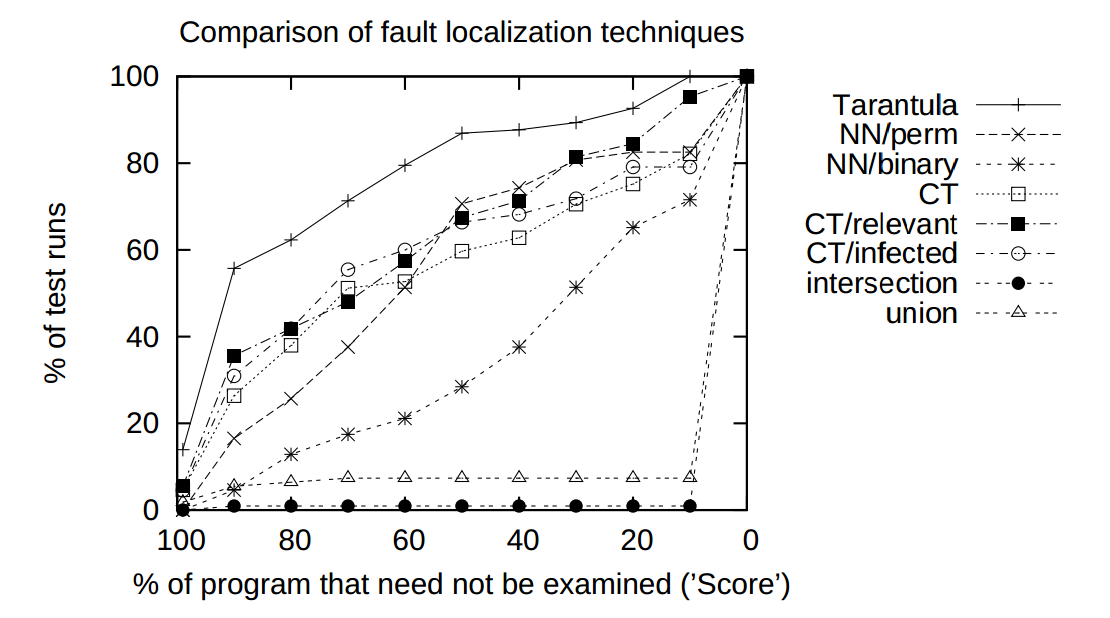
\includegraphics[width=0.9\linewidth]{img/tareff.png}
  \caption{An empirical comparison of several fault localization
  techniques by percentage of code eliminated from consideration.  The
  graph plots percentage eliminated (determined by the rank of the
  faulty statement) against frequency that the tool achieved that level
  of success.  Tarantula is demonstrated to achieve better results more
  often than other techniques.(from \cite{harrold})}
  \label{tareval}
\end{figure}

Xie et al. present an alternative discussion of various risk evaluation 
functions focusing primarily on theoretical correctness \cite{theory}. They 
argue that many existing risk evaluation formulas are actually functionally
equivalent.  In addition, they provide theoretical analysis that shows the 
superiority of specific functions relative to one another both within 
functionally equivalent groups and between those groups. Through detailed
theoretical proof they show that the equivalent sets ER1 and ER5 are maximal
for accurately calculating suspiciousness.  The ER1 set includes a pair of 
formulas studied in a paper by Naish et al. \cite{naish}  The ER5 equivalent 
set includes three functions, two of which are also studied in the paper
by Naish et al. The third is discussed in a paper by Wong et al. \cite{wong}
It is important to note that all the above risk evaluations also require
per-test coverage data.

As a followup to the paper by Xie et al. mentioned above, Qi et al. \hspace*{-0.7mm}\cite{genprog}
performed a detailed empirical to study the practical effectiveness of the 
theoretically maximal functions as proven by Xi et al.  This study includes
a wide variety of risk evaluation functions, and compares them by applying 
them to practical, real-world programs and faults.  The various formulas
were inserted into popular automated program repair system GenProg.
GenProg uses genetic programming, applying a risk evaluation function to 
repeatedly alter a faulty program by mutating suspicious statements.  In their
study, Qi et al. \hspace*{-0.5mm}modified GenProg to use several different formulas.  By 
comparing the effectiveness of automated repair when using each 
risk evaluation function, they were able to provide substantial empirical
evidence regarding the superiority of certain formulas.  Note that this method
of comparison differs from that pursued by Jones and Harrold \cite{harrold}, 
discussed previously, which compared the relative suspiciousness ranking of 
faulty statements (referred to as EXAM score).

Surprisingly, Qi et al. did not confirm the results shown by Xie et al.
Instead, they found that several functions, eliminated from consideration
as maximal functions early in the proof provided by Xie et al., were actually 
better than expected. Specifically,
Qi et al. show that in practice, the Jaccard risk evaluation function performed
as well or better than all other formulas considered.  They conclude that,
at least within the context of automated program repair, Jaccard should be 
favored when choosing a risk evaluation function.  In addition, they further 
conclude that the EXAM score method of comparing these formulas does not 
accurately reflect their relative performance in the context of automated
program repair.

In another paper \cite{parnin}, Parnin and Orso performed a human study on the
real-world effectiveness of fault localization techniques.  In that
study, they asked participants, graduate students in computer science
with varying levels of experience, to perform debugging tasks.
Participants were asked to compare their experiences when using standard
debugging practices with using an Eclipse plugin designed to display
Tarantula suspiciousness ranking.  This plugin was made as simple as possible
so as to only consider suspiciousness.  The only functionality provided was a list of suspicious statements
which, when selected, navigated the environment to that line in the source
code.  When evaluating their hypotheses, the authors considered the
relative average amount of time required for each task, with and without
the plugin.  They also considered the relative experience level of the 
participants, which they evaluated based on number of tasks completed.  In 
addition, they also experimented with artificially raising and lowering
the rank of the fault statement in the suspicious statement list.  Finally,
Parnin and Orso used their plugin to record the order in which users
visited the suspicious statements, and asked the participants to complete
a questionnaire about their experiences and use of the tool.

Parnin and Orso came to a number of conclusions regarding several different
comparisons.  First, they noticed that, in general, the participants did not
complete the tasks faster to any degree of statistical significance.  However,
they did notice a significant improvement in performance when using the tool
if the subject in question was more experienced.  This suggests that, if the
tool were more refined and participants more used to the tool, it might actually
be significantly more helpful.  They also found evidence that suggests that the
exact rank of the statement does not significantly affect the difficulty of
locating the fault when using the tool.  In particular, participants often 
navigated the list of statements in a non-linear fashion: sometimes they skipped
ahead or backwards.  When skipping ahead, the authors suggest that participants
may have been skipping over code blocks they had already deemed unlikely to contain
the bug.  Finally, they conclude that there is no such thing as perfect bug 
understanding in practice.  That is, simply seeing a faulty statement out of 
context is not sufficient to identify and repair the bug.

We notice first that a large number of the negative results from Parnin and Orso's
study, in regards to the effectiveness of automatic fault localization, may have
stemmed from the simplicity of the Eclipse plugin tested.  We therefore hypothesize
that with a more sophisticated tool, programmers will have significantly improved
performance over the use of traditional debugging techniques.  Since the goal of our
tool is to provide per-test coverage as context for suspiciousness, we suggest that
our tool is likely to outperform traditional debugging.

\section{CodeCover Coverage Analysis}\label{sec:cover}
CodeCover produces coverage information for Java, and has built in 
functionality for generating coverage information on a per-test suite,
per-test case, and even per-test method basis.  In addition, CodeCover
is designed to function within Eclipse.  All parts of the coverage
monitoring process can be done through the Eclipse development
environment.  Since the final goal of this project is to produce an
integrated Eclipse tool for fault localization, using per test
coverage and risk evaluation, CodeCover is ideally suited to our
purposes.  

\begin{figure}[htpb]
  \centering
  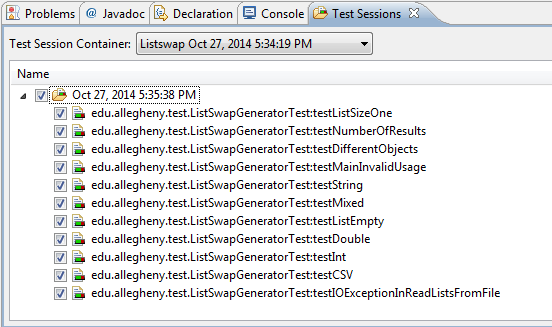
\includegraphics[width=4in]{img/codecoverpertest.png}
  \caption{Screenshot of CodeCover Eclipse plugin displaying per-test coverage
  output from a single execution of a JUnit test suite.}
  \label{codecover}
\end{figure}

CodeCover works in several stages.  The first step to acquiring coverage
information is instrumentation.  During instrumentation, numerous
statements are procedurally inserted into the Java source files which 
are to be included in the coverage analysis.  In the context of Eclipse,
these files are manually marked, since there may be source files for 
which coverage information is unnecessary.  The statements that are 
inserted during instrumentation record various information as the code
is executed, including which existing Java statements were executed, and
which test case or method executed them.  After instrumentation is
complete, the newly instrumented source files, as well as any other source
files, are compiled as normal.

CodeCover provides functionality for using existing JUnit test cases and
test suites for coverage analysis. With an existing Eclipse project with 
a JUnit test class, CodeCover can simply be enabled and executed.  By 
default, CodeCover produces output in the form of a several coverage
reports.  The output includes a full coverage report for every test method 
within the JUnit test; that is, per-test coverage data, as shown in Figure
\ref{codecover}.  

After executing a test process through the CodeCover Eclipse, per-test
coverage can be viewed in several ways.  First, coverage can be viewed on 
a per-test basis within Eclipse.  As shown in Figure \ref{codecoverage}, 
selecting one or more test methods displays coverage information for those
test methods only.  In addition to viewing coverage within Eclipse, CodeCover
allows coverage information to be executed in a variety of formats.  Using
provided template XML (eXtensible Markup Language) files, coverage data can be exported, for example, as
hierarchical HTML (HyperText Markup Language) documents or as CSV (Comma Separated Value) files.  

\begin{figure}[tpb]
  \centering
  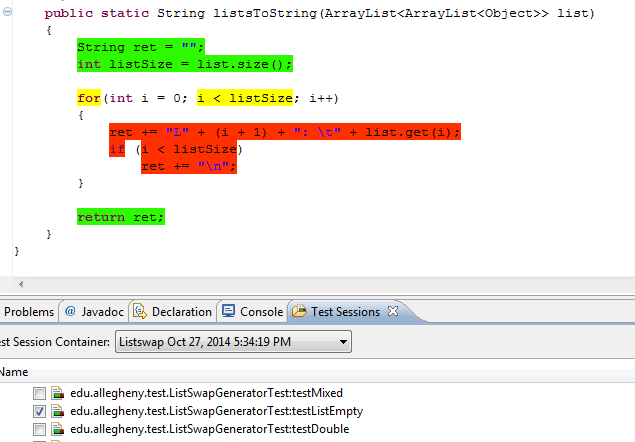
\includegraphics[width=4in]{img/codecovercoverage.png}
  \caption{Screenshot of CodeCover Eclipse plugin displaying coverage
  highlighting for a single test method.  Statements highlighted in green
  were covered by this test method, and those in red were not.}
  \label{codecoverage}
\end{figure}

\section{MAJOR Mutation}\label{sec:major}

MAJOR is a fault seeding and mutation analysis tool that integrates
directly into the Java compiler \cite{major}. \emph{Mutation} is the process of
intentionally introducing faults into a program for various purposes,
including evaluation of test suite quality and testing for fault
localization techniques.  Mutants generated are either \emph{killed} by
the test suite or \emph{live}.  A mutant is killed if a test case fails;
that is, the test suite was sufficient to identify the fault.  Live
mutants either indicate that the test suite is insufficient or that the
introduced fault was in fact logically equivalent to the original code.

MAJOR can perform a number of conditional mutations, including replacing
binary arithmetic, logical, relational, shift and unary operators with
valid alternatives.  One example of a possible mutation performed by
MAJOR is shown in Figure \ref{majorex}.  The tool can also replace literal
values with alternatives; these various mutation types can be selected
with compiler operators.  Along with the domain specific language
provided by MAJOR, this allows for great flexibility and extensibility.
Additionally, MAJOR has been shown to be relatively efficient, with only
about 15\% runtime overhead.  It is also noteworthy that MAJOR utilizes
coverage analysis to improve efficiency.

A recent paper by Just et al. \cite{mutants} indicates a statistical
correlation between mutant detection and real world fault detection.
Although they also note that as much as 20\% of real world faults cannot
be represented by mutants, this still suggests that mutants are a viable
substitute for real world faults in the context of software testing and,
similarly, fault localization.

\begin{figure}[tbp]
  \centering
  \begin{lstlisting}
public static Type classify(int a, int b, int c) {
		int trian;
		if (a <= 0 || b <= 0 || c <= 0)
			return Type.INVALID;
		trian = 0;
	        ... (additional statements) ...
}
\end{lstlisting}

  \begin{lstlisting}
public static Type classify(int a, int b, int c) {
		int trian;
		if ((a <= 0 || b <= 0) != c <= 0)
			return Type.INVALID;
		trian = 0;
	        ... (additional statements) ...
}
\end{lstlisting}

  \caption{(top) Original program and (bottom) program after mutation.}
  \label{majorex}
\end{figure}